%\documentclass[t,10pt]{beamer}
\documentclass[t,handout]{beamer}

\usepackage{graphicx}
\usepackage{epsfig}
\usepackage{psfrag}
\usepackage[english]{babel}
\usepackage{color}
\usepackage{natbib}



%\usepackage[latin1]{inputenc}
%\usepackage{amsmath}
%\usepackage{amsfonts}
%\usepackage{amssymb}
%\usepackage{graphicx}
%\usepackage{epsfig}
\usepackage{booktabs}
\usepackage{listings}
%\usepackage{courier}
%\usepackage{multirow}
%\usepackage{color}
%\usepackage{framed}
%\usepackage{lipsum}

% Font settings:
\usepackage[T1]{fontenc}
%\usepackage{mathpazo}
\usepackage{mathptmx}
\usepackage[scaled]{helvet}
\usepackage{courier}
\usepackage{microtype}



%Mathematics packages
\usepackage{amsmath}
\usepackage{mathrsfs}
\usepackage{amsfonts}
\usepackage{enumerate}

\graphicspath{{./images/}} % Figures path - used in graphicx

\selectcolormodel{cmyk}

\mode<presentation>

%THEMES - Please refer to these chapters in the beamer documentation.
% Presentation themes : Chapter 15
% Color themes : Chapter 17
% Font themes : Chapter 18
\usetheme{Pittsburgh}
\usecolortheme{orchid}
\usefonttheme{default}

\setbeamertemplate{bibliography item}[text]
\setbeamercovered{transparent=7}

%---------------------------Title frame definition------------------------------------- 

\title{Information Protection in Content-centric Networks}
\author [Chris]{Christopher C. Lamb}
\institute[University of New Mexico]{
\inst {}Department of Electrical and Computer Engineering\\
University of New Mexico}
\date{November 6, 2012}
\titlegraphic{
\begin{figure} 

\includegraphics[width = 7cm]{UNM}
\end{figure}}

% Delete this, if you do not want the table of contents to pop up at
% the beginning of each subsection:
%\AtBeginSubsection[]
%{
%  \begin{frame}<beamer>
%    \frametitle{Outline}
%     \tableofcontents[currentsection,currentsubsection]
%  \end{frame}
%}

\begin{document}

\begin{frame}
\titlepage
\end{frame}

% This command will make the logo appear on all frames excluding the title frame.
\logo {
\includegraphics[width = 2.5cm]{UNM}}

\begin{frame}[t]
\frametitle{Outline}
\tableofcontents 
\end{frame}

%\section{Summary Results}

\begin{frame}
\frametitle{Conclusions}
\begin{beamerboxesrounded}[shadow]{Contribution of Work}
The contribution of this work is a quantitative analysis of policy-centric overlay network options, associated taxonomies of use, and prototypical technology proofs-of-concept.
\end{beamerboxesrounded}
\begin{itemize}
\item \textit{Network Control Options} --- This includes various types networks and associated strengths and weaknesses addressing centralized and decentralized models.
\item \textit{Taxonomies of Use} --- Depending on the specific usage management requirements and context, different overlays have different applicability; this work will provide guidance on suitability; it will eventually lead to how to manage data flow within SDN-capable infrastructure.
\item \textit{Prototypical Technologies} --- Examples and proofs-of-concept will be required to appropriately analyze various architectural alternatives.
\end{itemize}
\end{frame}

\section{Summary}

\begin{frame}
\frametitle{Original Goals}
\begin{beamerboxesrounded}[shadow]{Contribution of Work}
The contribution of this work is a quantitative analysis of policy-centric overlay network options, associated taxonomies of use, and prototypical technology proofs-of-concept.
\end{beamerboxesrounded}
\begin{itemize}
\item \textit{Network Control Options} --- {\small This includes various types networks and associated strengths and weaknesses addressing centralized and decentralized models.}
\item \textit{Taxonomies of Use} --- {\small Depending on the specific usage management requirements and context, different overlays have different applicability; this work will provide guidance on suitability; it will eventually lead to how to manage data flow within SDN-capable infrastructure.}
\item \textit{Prototypical Technologies} --- {\small Examples and proofs-of-concept will be required to appropriately analyze various architectural alternatives.}
\end{itemize}
\end{frame}

\begin{frame}
\frametitle{Meeting the Goals}
\begin{beamerboxesrounded}[shadow]{Network Control Options}
{\small I have developed and analysed multiple types of overlay systems, both centralized (hierarchical) and non-centralized (non-hierarchical), with differing topologies and integrated content-centric control.}
\end{beamerboxesrounded}
~\\
\begin{beamerboxesrounded}[shadow]{Taxonomies of Use}
{\small I have established an verified a taxonomy of usage management and applied that within the network providing mechanisms extendable to SDN use.}
\end{beamerboxesrounded}
~\\
\begin{beamerboxesrounded}[shadow]{Prototypical Technologies}
{\small Prototype information-centric networks are running between the Rackspace and Amazon clouds.}
\end{beamerboxesrounded}
\end{frame}

\begin{frame}
\frametitle{Impact and Originality}
\begin{itemize}
\item Information-centric architectures common in future internet designs
\item Significant work with respect to name/object binding, overall topologies, approaches
\item No significant work yet on exploiting information-centricity for enhanced security
\item They have significant new capabilities inherent in approach that allow for better information security
\end{itemize}
\begin{beamerboxesrounded}[shadow]{Additional Contributions}
{\small This work, as well as providing alternatives analysis with respect to information-centric security with respect to architectures and approaches, also demonstrates the first implementation of granular context-sensitive security functionality embedded in an information-centric network.}
\end{beamerboxesrounded}
\end{frame}

\begin{frame}
\frametitle{Publications (current)}
{\bf Conference Papers:} \\
\begin{scriptsize}
C.C. Lamb and G.L. Heileman. Overlay architectures enabling cloud computing for multi-level security environments. In Services (SERVICES), 2012 IEEE Eighth World Congress on, pages 116-124, june 2012.\\
~\\
Christopher Charles Lamb, Pramod A. Jamkhedkar, Mathew P. Bohnsack, Viswanath Nandina, and Gregory L. Heileman. {\sl A domain specific language for usage management}. In Proceedings of the 11th annual ACM workshop on Digital rights management, DRM '11, pages 51-62, New York, NY, USA, 2011. ACM. \\
~\\
Christopher C. Lamb, Pramod A. Jamkhedkar, Gregory L. Heileman, and Chaouki T. Abdallah. {\sl Managed control of composite cloud systems}. In System of Systems Engineering (SoSE), 2011 6th International Conference on, pages 167-172, june 2011. \\
~\\
P.A. Jamkhedkar, C.C. Lamb, and G.L. Heileman. {\sl Usage management in cloud computing}. In Cloud Computing (CLOUD), 2011 IEEE International Conference on, pages 525-532, july 2011. \\
~\\
Pramod A. Jamkhedkar, Gregory L. Heileman, and Chris C. Lamb. {\sl An interoperable usage management framework}. In Proceedings of the tenth annual ACM workshop on Digital rights management, DRM '10, pages 73-88, New York, NY, USA, 2010. ACM. \\
~\\
\end{scriptsize}
\end{frame}

\begin{frame}
\frametitle{Publications (submitted)}
{\bf Journal Submissions:} \\
\begin{scriptsize}
C.C. Lamb and G.L. Heileman. Overlay architectures enabling cloud computing for multi-level security environments. In Services (SERVICES), 2012 IEEE Eighth World Congress on, pages 116-124, june 2012.\\
~\\
Christopher Charles Lamb, Pramod A. Jamkhedkar, Mathew P. Bohnsack, Viswanath Nandina, and Gregory L. Heileman. A domain specific language for usage management. In Proceedings of the 11th annual ACM workshop on Digital rights management, DRM '11, pages 51-62, New York, NY, USA, 2011. ACM. \\
~\\
\end{scriptsize}
{\bf Book Chapters:} \\
\begin{scriptsize}

\end{scriptsize}
\end{frame}

\section{Results Summary}

\begin{frame}
\frametitle{Results Overview}
Overall evaluation of impact against strategy:
\begin{itemize}
\item {\small Encryption most likely to be used...}
\item {\small ...Rerouting likely the best compromise (but expensive)}
\item {\small Hierarchical and non-hierarchical networks had similar performance}
\item {\small No clear leading strategy under all conditions}
\end{itemize}
~\\
\centering %
\begin{tabular}{lccc}
\toprule %
{\bf Property}			& {\bf Redaction}	& {\bf Rerouting} 	& {\bf Encryption} 	\\\toprule
{\bf Confidentiality} 	& 3				  	& 2					& 1				 	\\\midrule
{\bf Integrity}			& 0					& 1					& 3 					\\\midrule
{\bf Availability}		& 0					& 1					& 2					\\\bottomrule
\end{tabular}
\label{table:model:evaluation}
\begin{center}
{\small Strategy Impact by Attribute}
\end{center}
\begin{center}
{\bf What does this mean? How did we get it?}
\end{center}
\end{frame}

\begin{frame}
\frametitle{Methodology}
{\bf \textit{Confidentiality, Integrity characteristics based on approach.}} \\
\begin{itemize}
\item {\small {\bf Redaction}, by removing information, by definition destroys integrity while guaranteeing confidentiality; unavailable information that is cannot be leaked}
\item {\small {\bf Rerouting} removes information from a context damaging integrity that can possibly be repaired later, potentially increasing confidentiality by rendering that information unavailable}
\item {\small {\bf Encryption} minimizes integrity impacts be keeping ciphered data with original context at the expense of possible interception and cryptanalysis exposure}
\end{itemize}
{\bf \textit{Availability is based on performance.}} \\
\begin{itemize}
\item {\small {\bf Performance} is measured via end-to-end time of transmittal}
\end{itemize}
\end{frame}

\begin{frame}
\frametitle{Redaction}
{\bf Redaction:} {\small Removing content that is not approved for transmission over a given link or consumption by a given agent from a larger context of suitable content.} \\
\begin{itemize}
\item {\small Strongest confidentiality}
\item {\small Destroys integrity}
\item {\small Mixed impact on availability}
\end{itemize}
\begin{center}
{\bf \textit{Fast and easy to implement}}
\\~\\
\begin{small}
\begin{tabular}{lccc}
\toprule %
{\bf Property}			& {\bf Redaction}	& {\bf Rerouting} 	& {\bf Encryption} 	\\\toprule
{\bf Confidentiality} 	& 3				  	& 2					& 1				 	\\\midrule
{\bf Integrity}			& 0					& 1					& 3 					\\\midrule
{\bf Availability}		& 0					& 1					& 2					\\\bottomrule
\end{tabular}
\end{small}
\end{center}
\end{frame}

\begin{frame}
\frametitle{Rerouting}
{\bf Rerouting:} {\small Removing content that is not approved for transmission over a given link and rerouting that content to its destination through secondary means (e.g. SMTP).} \\
\begin{itemize}
\item {\small Confidentiality dependent on secondary links}
\item {\small Integrity compromised temporarily and perhaps permanently}
\item {\small Availability dependent on secondary links}
\end{itemize}
\begin{center}
{\bf \textit{Undependable, expensive, good information control}}
\\~\\
\begin{small}
\begin{tabular}{lccc}
\toprule %
{\bf Property}			& {\bf Redaction}	& {\bf Rerouting} 	& {\bf Encryption} 	\\\toprule
{\bf Confidentiality} 	& 3				  	& 2					& 1				 	\\\midrule
{\bf Integrity}			& 0					& 1					& 3 					\\\midrule
{\bf Availability}		& 0					& 1					& 2					\\\bottomrule
\end{tabular}
\end{small}
\end{center}
\end{frame}

\begin{frame}
\frametitle{Encryption}
{\bf Encryption:} {\small Enciphering content within larger documents, deciphering enciphered sections when suitable by defined policy and when content needs to be re-evaluated.} \\
\begin{itemize}
\item {\small Confidentiality questionable over time}
\item {\small Integrity compromised temporarily and perhaps permanently}
\item {\small Availability dependent on secondary links}
\end{itemize}
\begin{center}
{\bf \textit{Reasonably secure, simple and performant}}
\\~\\
\begin{small}
\begin{tabular}{lccc}
\toprule %
{\bf Property}			& {\bf Redaction}	& {\bf Rerouting} 	& {\bf Encryption} 	\\\toprule
{\bf Confidentiality} 	& 3				  	& 2					& 1				 	\\\midrule
{\bf Integrity}			& 0					& 1					& 3 					\\\midrule
{\bf Availability}		& 0					& 1					& 2					\\\bottomrule
\end{tabular}
\end{small}
\end{center}
\end{frame}

\section{Test Network Topologies}

\begin{frame}
\frametitle{Physical Topology}
\begin{figure}[!t]
\centering
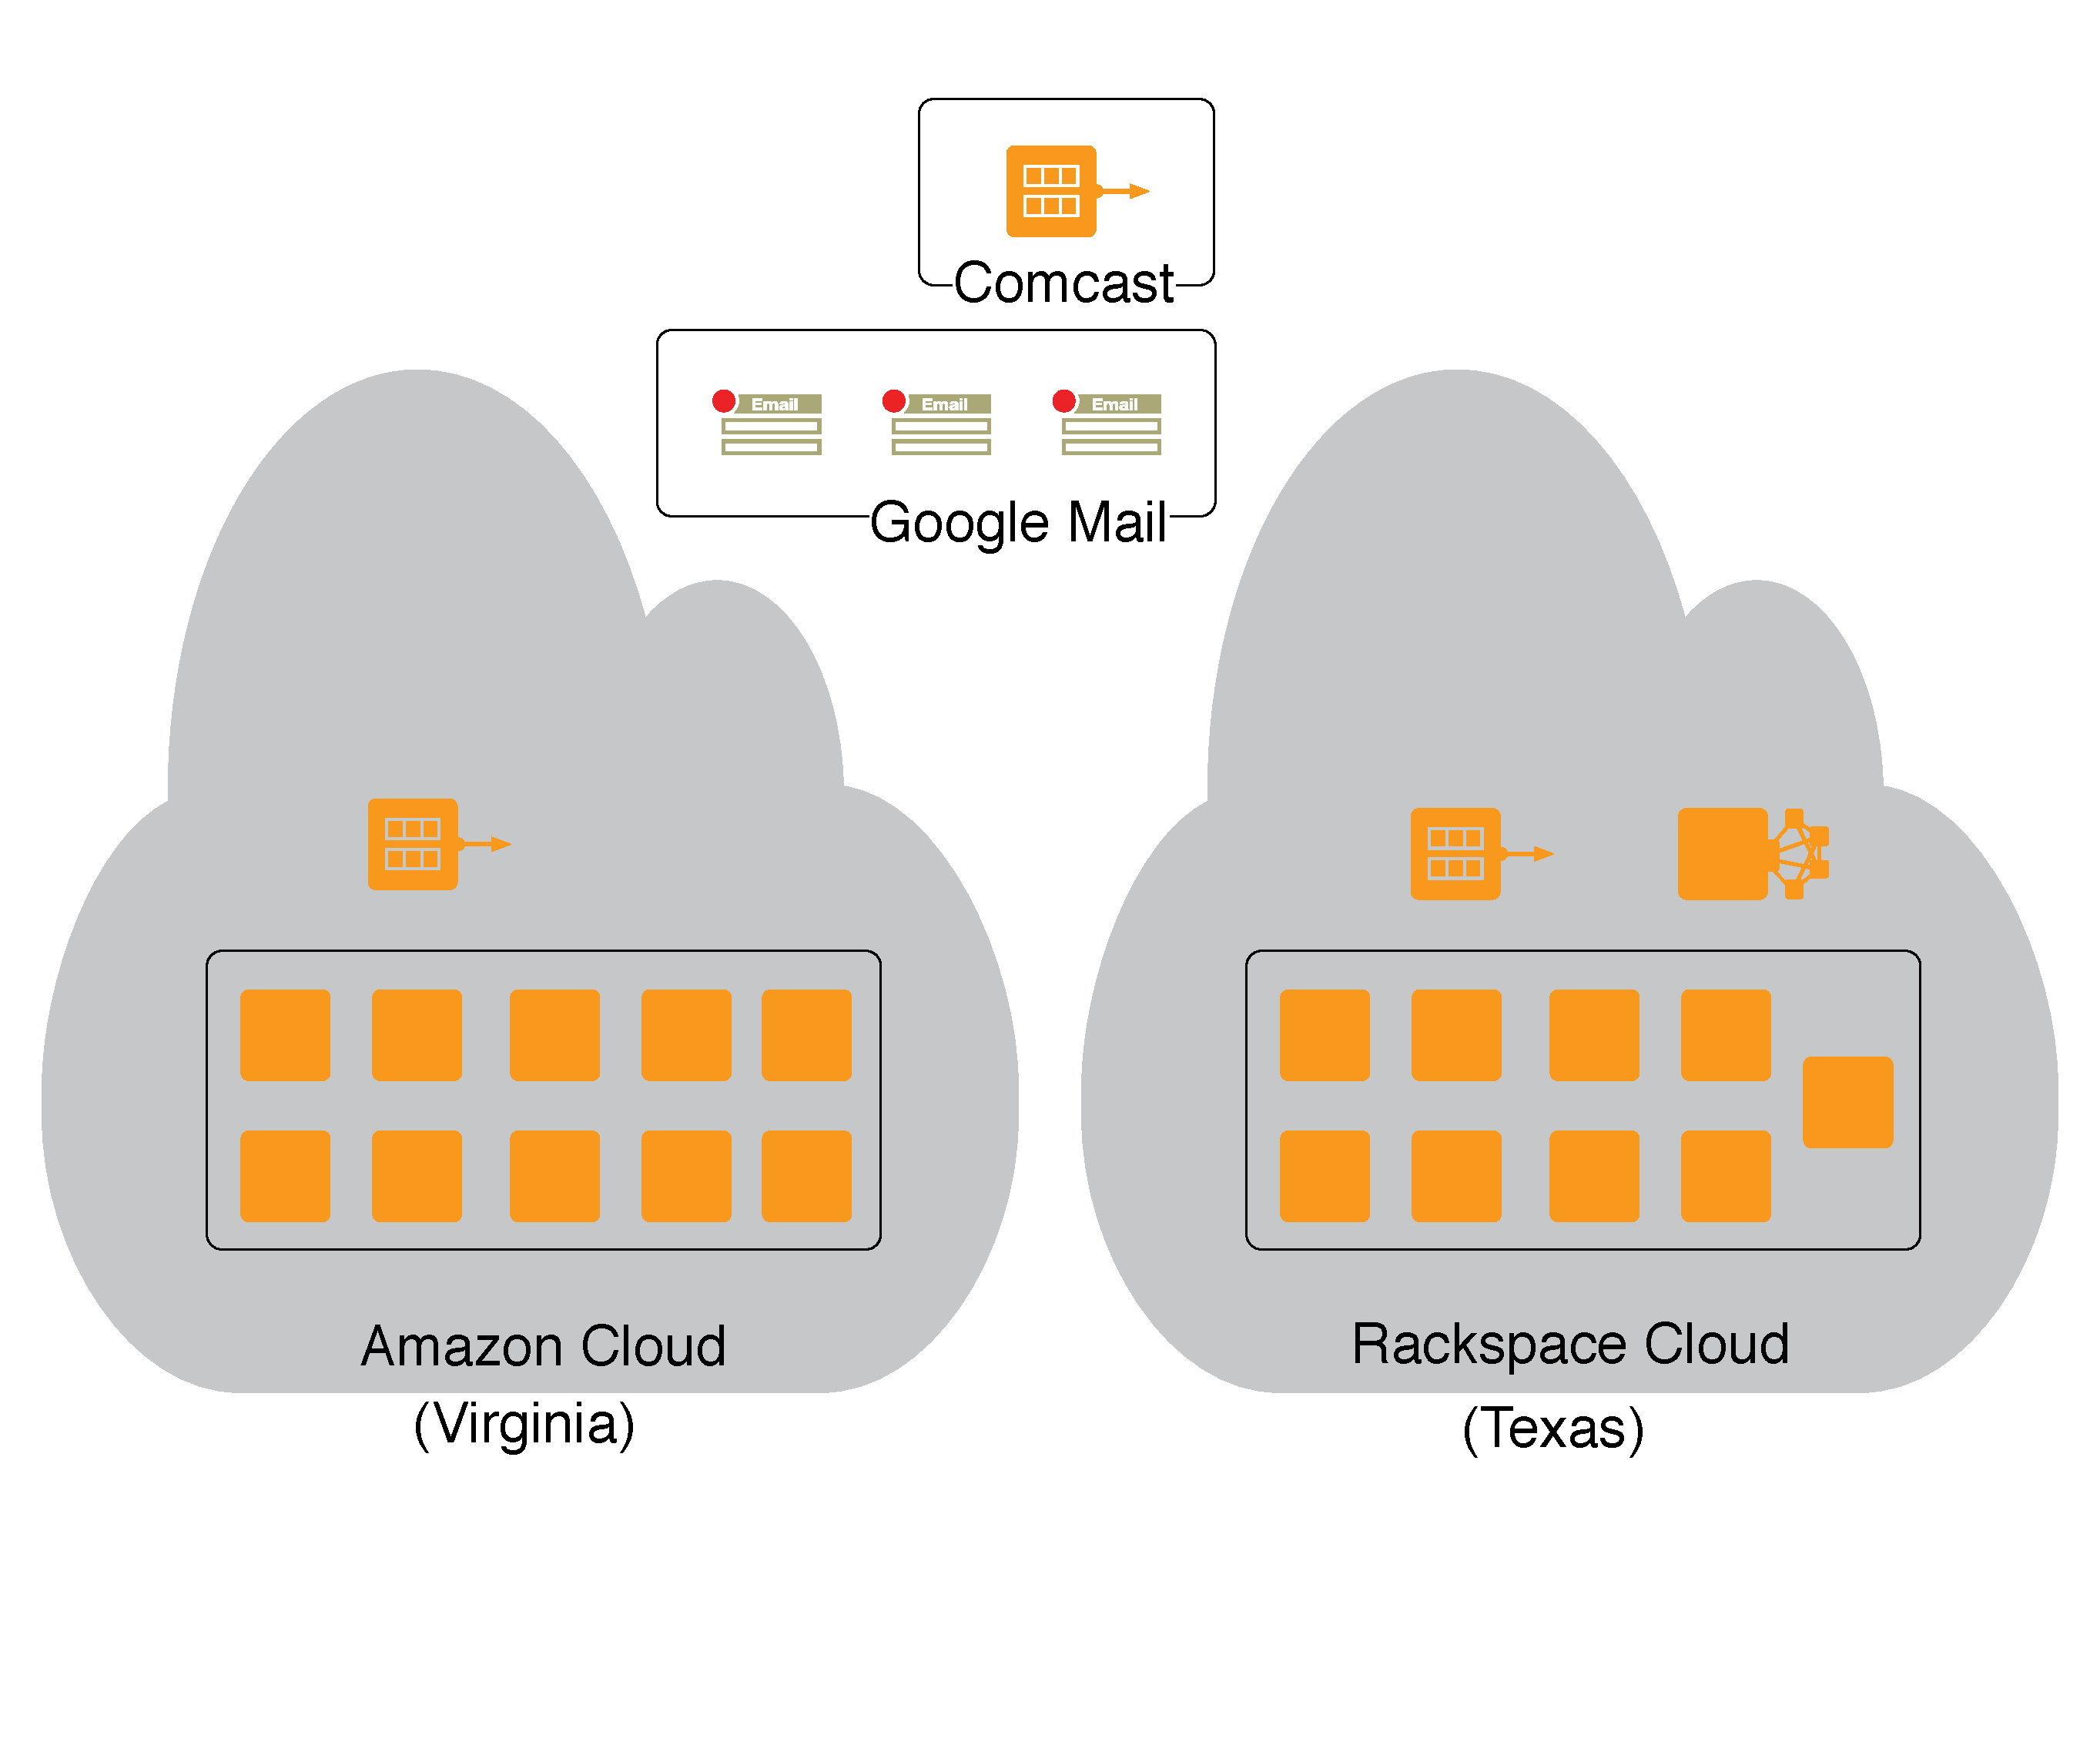
\includegraphics[width=3in]{physical-clouds}
\end{figure}
\end{frame}

\begin{frame}
\frametitle{Hierarchical Topology}
\begin{figure}[!t]
\centering
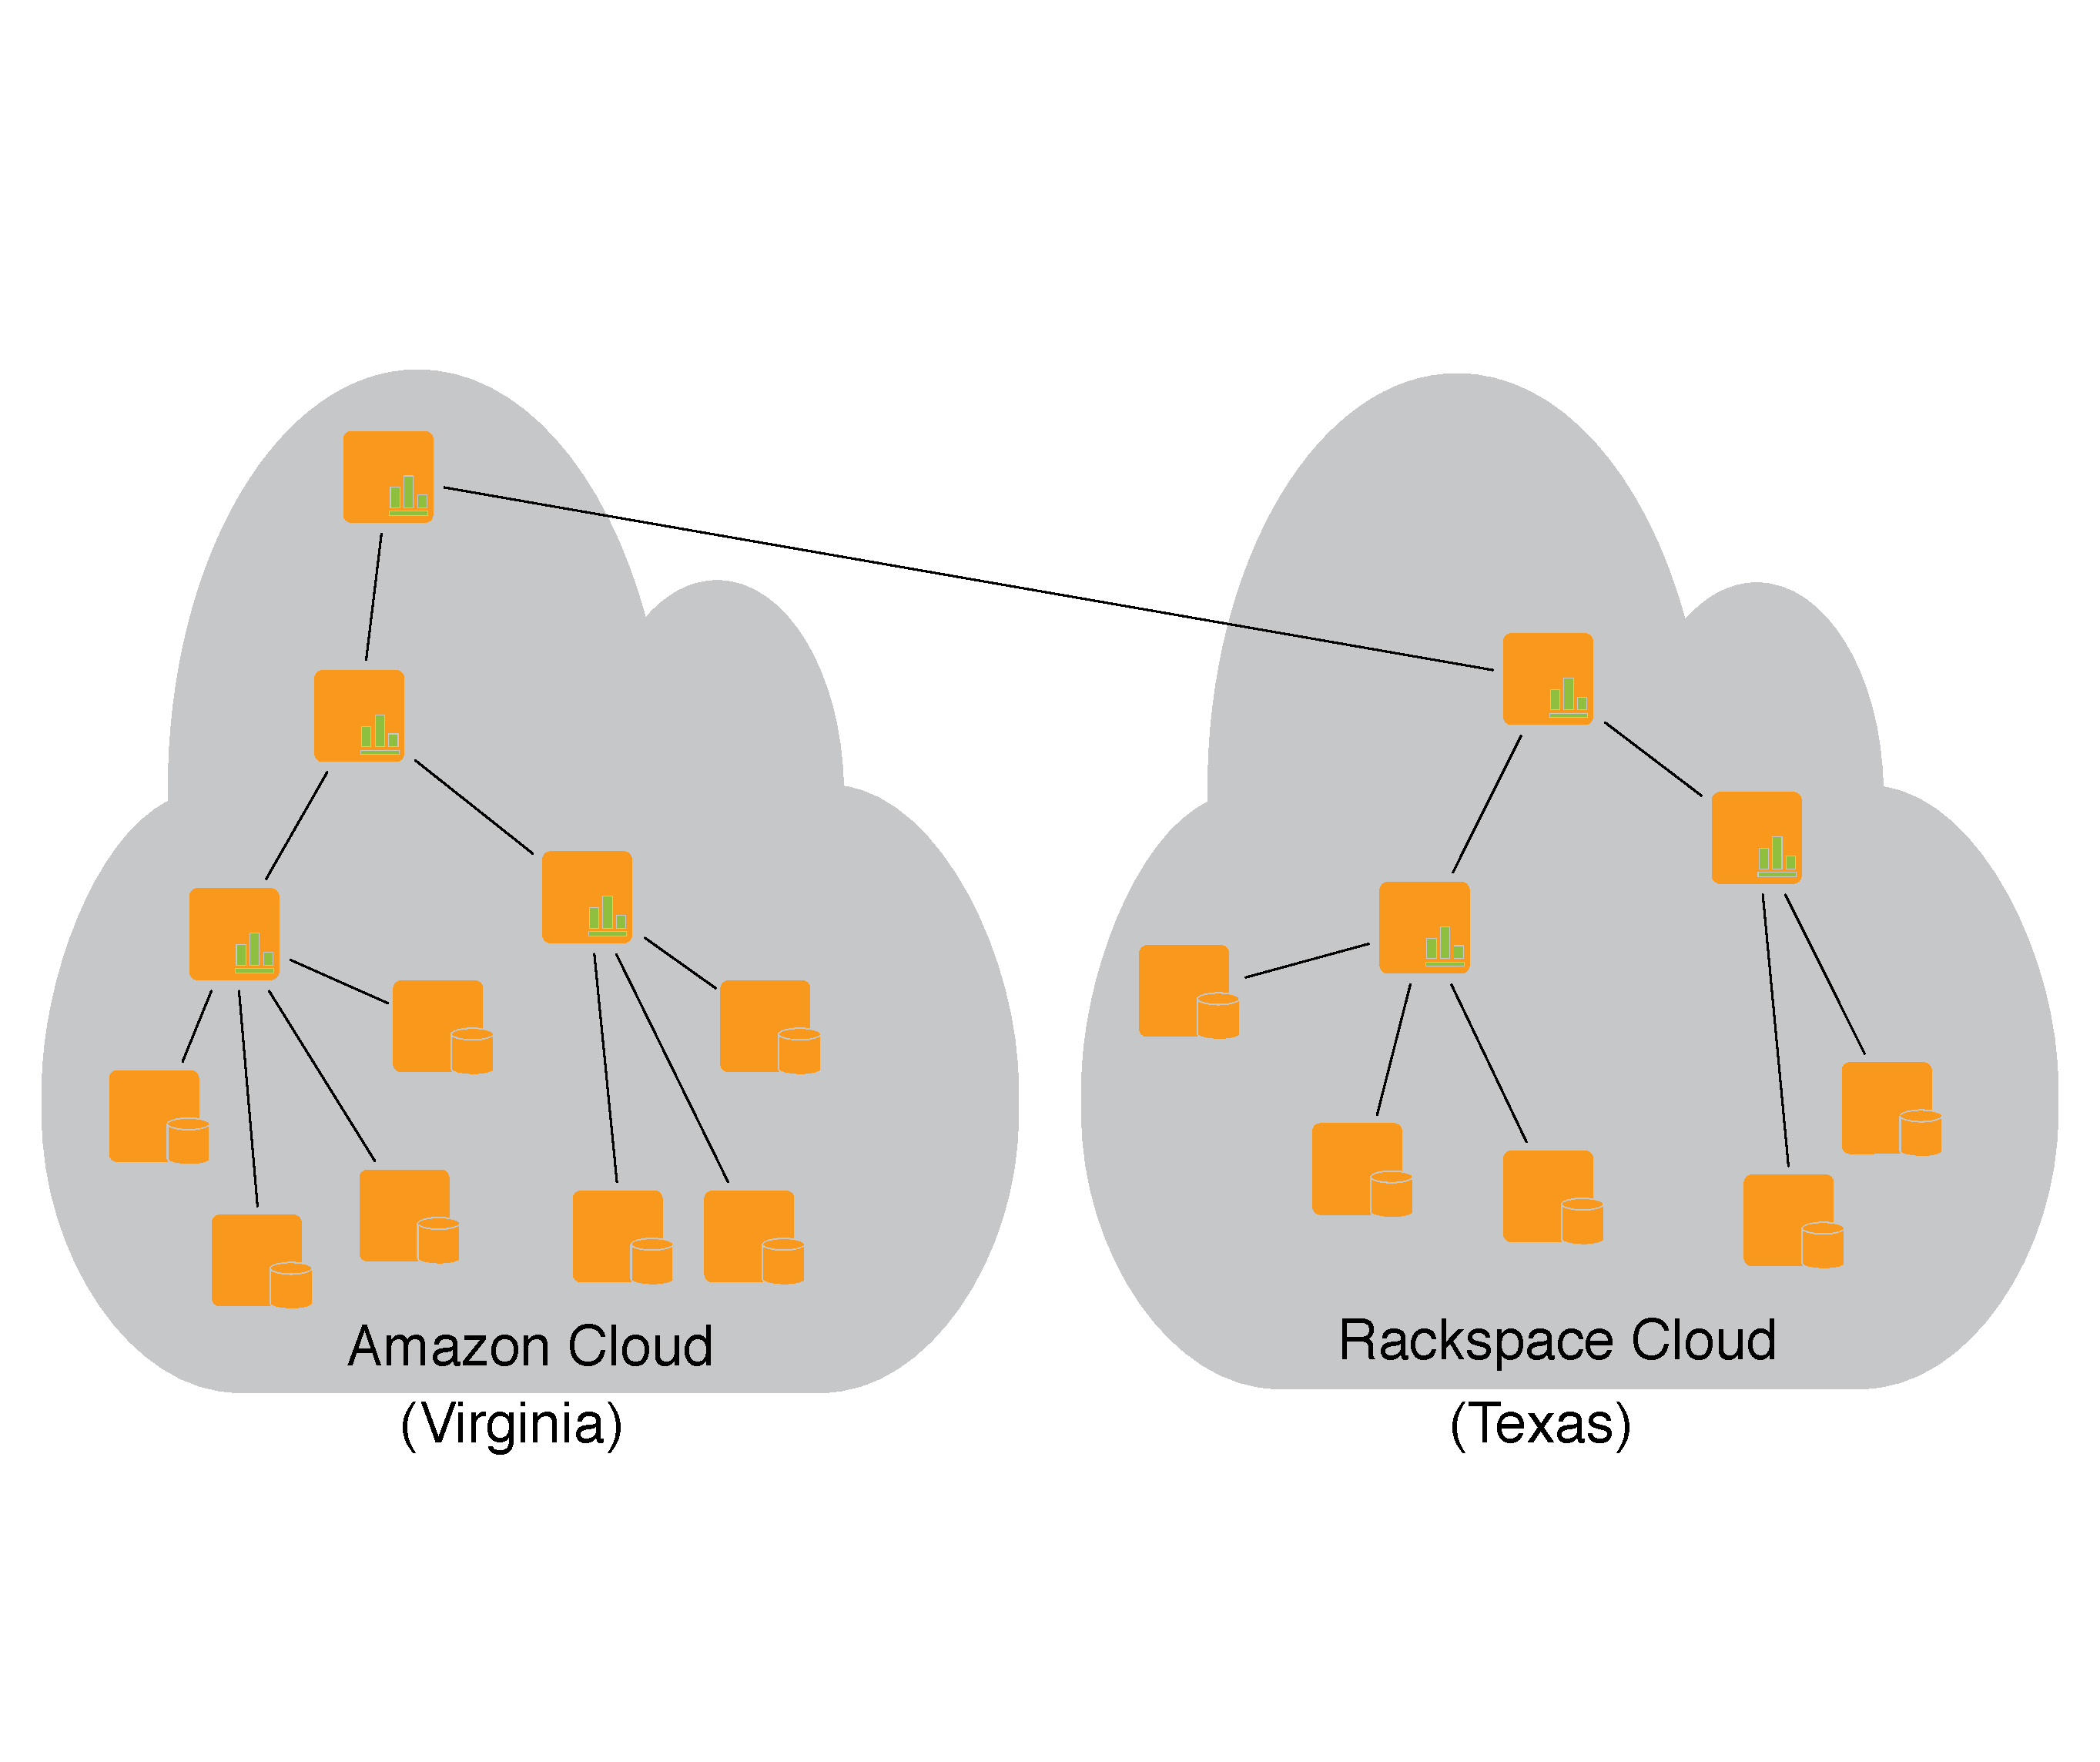
\includegraphics[width=3in]{hierarchical-clouds}
\end{figure}
\end{frame}

\begin{frame}
\frametitle{Non-Hierarchical Topology}
\begin{figure}[!t]
\centering
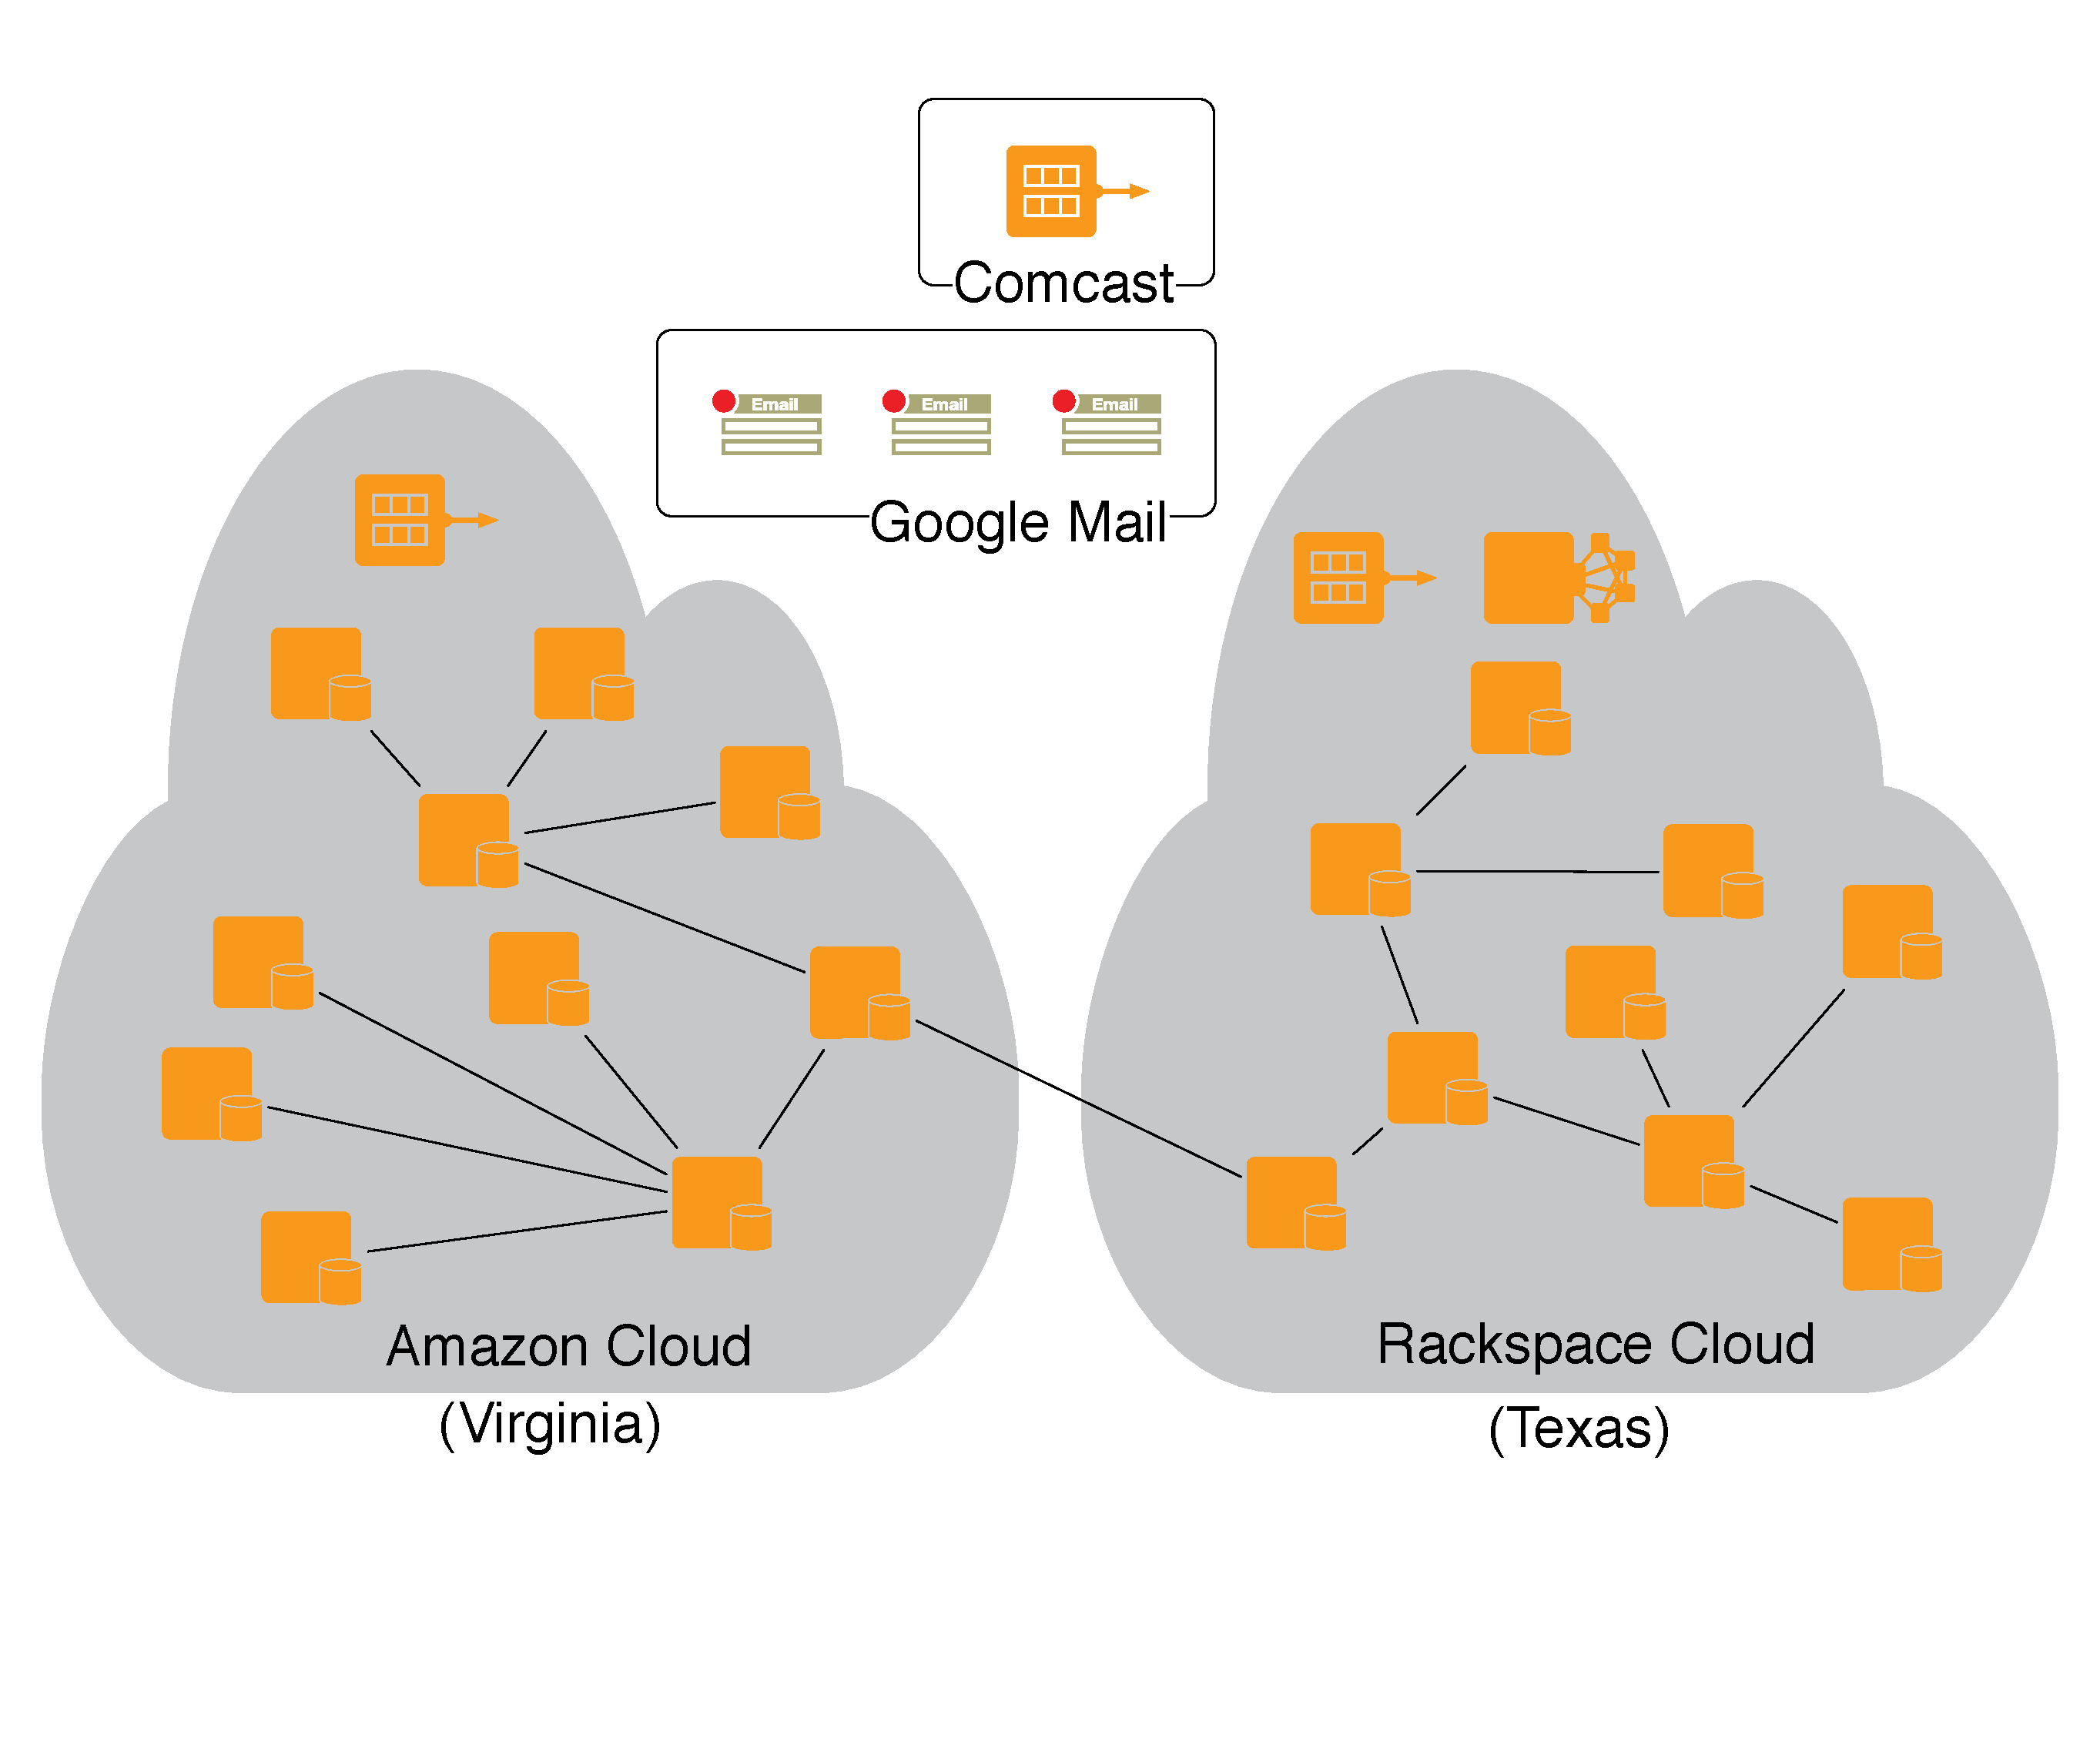
\includegraphics[width=3in]{non-hierarchical-clouds}
\end{figure}
\end{frame}

\section{Results Detail}

\begin{frame}
\frametitle{Hierarchical Effects}
\begin{figure}[!t]
\centering
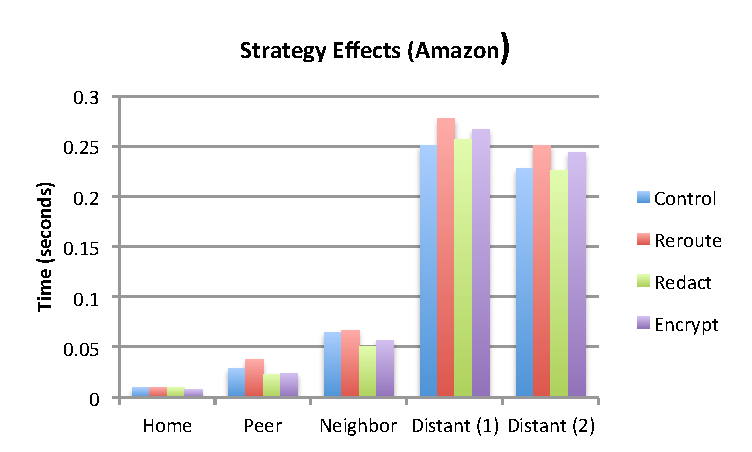
\includegraphics[width=4in]{strategy_effects_az}
\caption{Hierarchical Results from Amazon}
\end{figure}
\end{frame}

\begin{frame}
\frametitle{Hierarchical Effects}
\begin{figure}[!t]
\centering
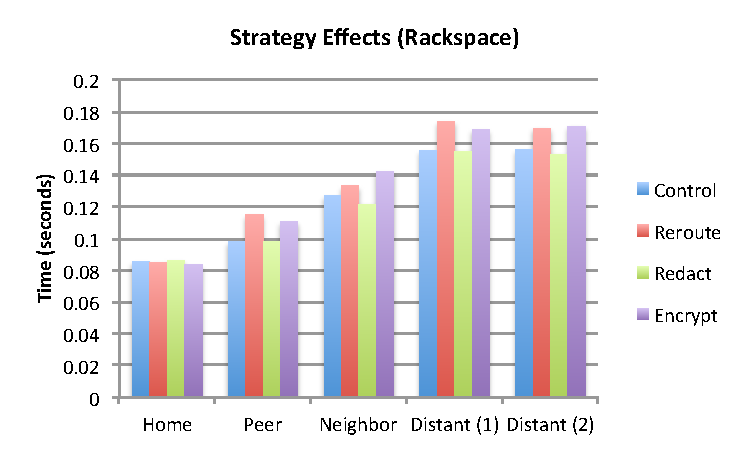
\includegraphics[width=4in]{strategy_effects_rs}
\caption{Hierarchical Results from Rackspace}
\end{figure}
\end{frame}

\begin{frame}
\frametitle{Hierarchical Effects}
\begin{figure}[!t]
\centering
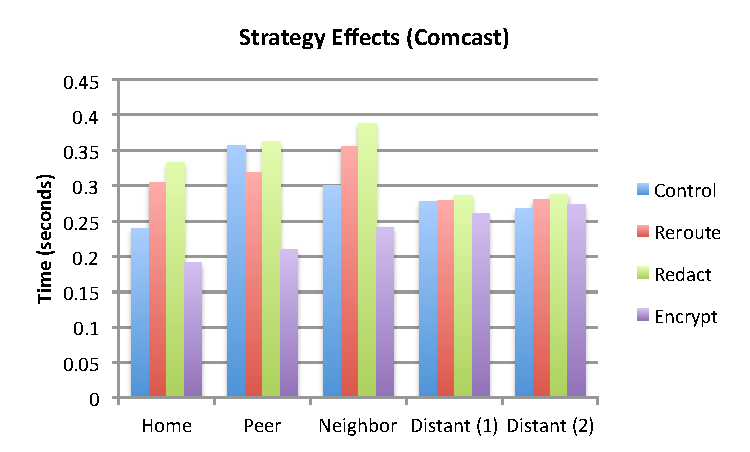
\includegraphics[width=4in]{strategy_effects_local}
\caption{Hierarchical Results from Comcast}
\end{figure}
\end{frame}

\begin{frame}
\frametitle{Hierarchical Analysis}

\end{frame}

\begin{frame}
\frametitle{Non-Hierarchical Effects}
\begin{figure}[!t]
\centering
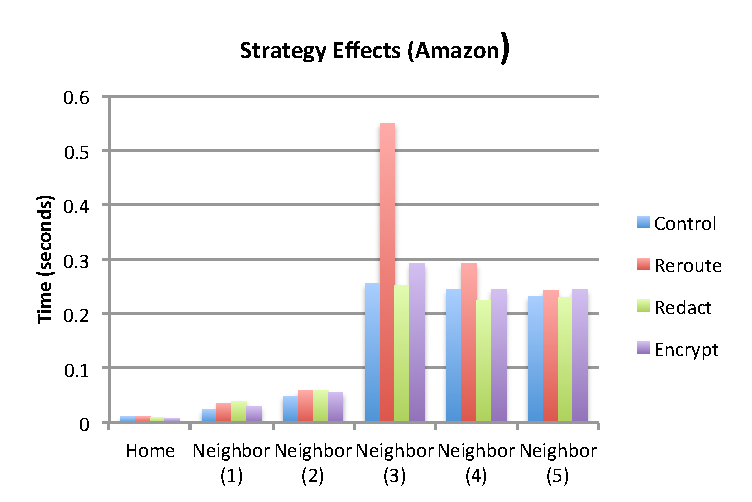
\includegraphics[width=4in]{nh_strategy_effects_az}
\caption{Non-Hierarchical Results from Amazon}
\end{figure}
\end{frame}

\begin{frame}
\frametitle{Non-Hierarchical Effects}
\begin{figure}[!t]
\centering
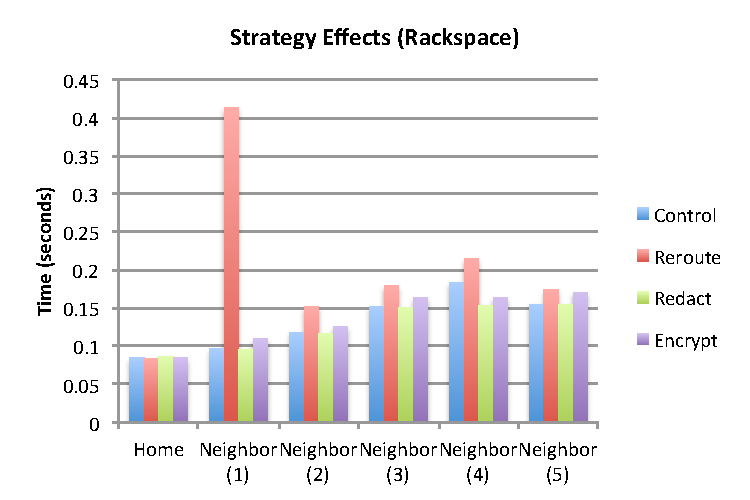
\includegraphics[width=4in]{nh_strategy_effects_rs}
\caption{Non-Hierarchical  Results from Rackspace}
\end{figure}
\end{frame}

\begin{frame}
\frametitle{Non-Hierarchical Effects}
\begin{figure}[!t]
\centering
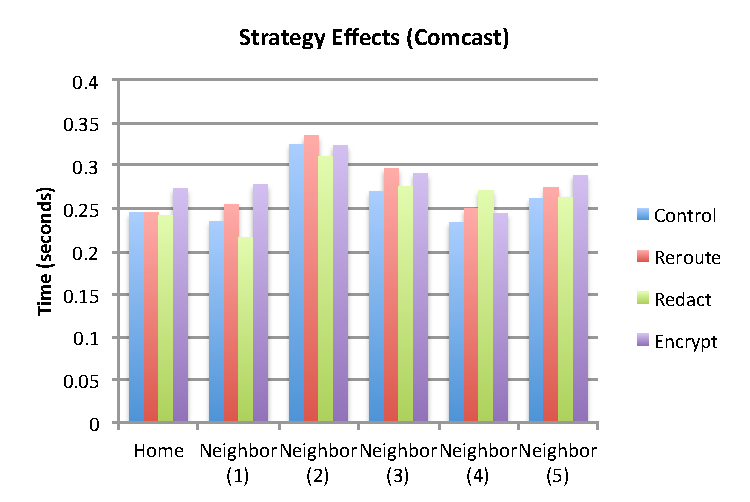
\includegraphics[width=4in]{nh_strategy_effects_local}
\caption{Non-Hierarchical Results from Comcast}
\end{figure}
\end{frame}

\begin{frame}
\frametitle{Non-Hierarchical Analysis}

\end{frame}

\begin{frame}
\frametitle{Network-Free Evaluation}
\begin{figure}[!t]
\centering
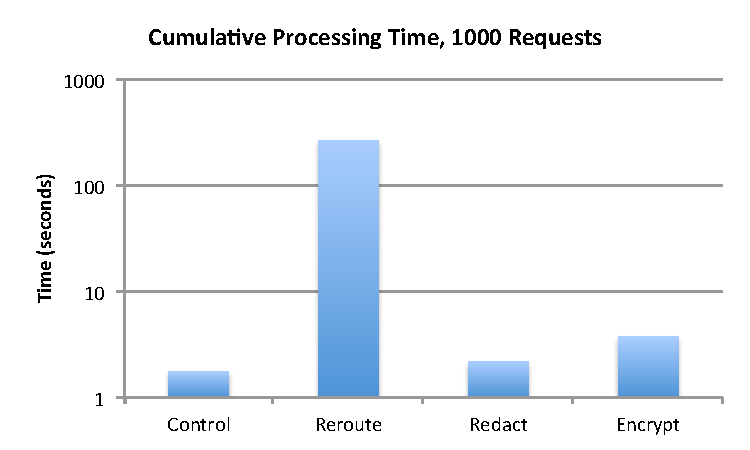
\includegraphics[width=4in]{single-node-results}
\caption{Results from Requests to a Singe Node}
\end{figure}
\end{frame}

\begin{frame}
\frametitle{Network-Free Analysis}

\end{frame}


%Experiments using this inter-cloud framework yield promising support for this approach.  They show only a slight degradation of information availability as a result of this network permeated security approach, with redaction and encryption demonstrating the smallest degradation at a higher impact on delivered information integrity.  Rerouting-based approaches have the most performance degradation. Encryption generally has the smallest impact on information integrity.  This is most evident when network effects are removed from evaluation.  Non-hierarchical and hierarchical networks have very similar performance with respect to content availability as well.

The goal of this experimental work was to characterize confidentiality, integrity, and availability impacts of these information-centric network security approaches in both hierarchical and non-hierarchical configurations.  The specific strategies addressed were redaction, rerouting, and protection (via encryption), and these strategies were evaluated from the perspective of confidentiality, integrity, and availability over hierarchical and non-hierarchical networks, and on standalone nodes. Confidentiality was measured via the control used to protect information.  Removing information entirely provided the highest measure of protection but is akin to unplugging a computer to improve its cyber-security posture.   Routing information through a more secure channel is the next most powerful approach, followed by sensitive information protection via strong encryption.  A 256-bit AES-CBC encryption scheme was used in this work.  Availability was measured by the delivery of information and the time required to ensure information delivery, measured by end-to-end network performance.  Integrity is a function of the alterations to the information required for secure delivery in the tested scenario.  Unaltered information has the highest integrity, followed by information that is still complete but protected via encryption, information that has been divided and rerouted, and finally information that has had content redacted.  Though combinations of strategies in a given network can be specified, as strategies are specified by network node, in these experiments only a single strategy in each network was used to more clearly attribute strategy performance impacts. Identical policies were used in each simulation to ensure the same amount of required usage management actions, limiting the effects on availability to the approach rather than differing policy.  In each case, a control simulation that did not incorporate any usage management was run to provide a performance baseline.  

\section{Hierarchical Networks}
In these tests, a simulated $\gamma$-categorized system was examined.  This is the kind of system that organizations like the UCDMO have identified as the final goal state of their work, systems that incorporate policy-centric management in the fabric of systems and networks (12).  The kind of components required to do this kind of policy-based content-sensitive evaluation do not currently exist, and components of these kinds of systems are only now beginning to emerge.  Systems like OpenFlow, when they have stronger hardware support, can begin to provide some of these kinds of capabilities.  OpenFlow enabled systems are not yet common or widely used however, and though they do provide the needed control for these kinds of systems, the do not supply the necessary policy interpretation and evaluation.  As a result, this experimental work was conducted over an HTTP overlay network, at the application layer.  Using a document-focused protocol makes content evaluation simpler as well, as systems can evaluate all content when it transits a network rather than maintaining a buffer of content required when processing packet-level communications.

In order to develop a stronger perspective on the network performance, delivery times were measured from three separate nodes.   One node is hosted in Comcast's infrastructure (a large local internet service provider), one at Amazon, and another at Rackspace.  The tested network had four levels.  The first level had a single router node.  The next level had two routers, both connected to the router in the first level.  The third level contained four routers, two attached to each of the routers at the level just above.  Finally, the fourth level contained nodes, distributed so that two level three routers had three nodes, one level three router had two nodes, and the last level three router had four nodes.  The first three levels were essentially a binary tree.  The network was queried from five different locations.  The node that contains the content was queried directly (the home node).  A node under the same router as the home node was then queried for content (the peer node).  Next, queries were sent to a node under a different router, but connected to the same second level router (the neighbor node).  Finally, two nodes on the other side of the network were queried for content (the distant (1) and (2) nodes).  Each node was queried for content 50 times in each simulation, for a total of 250 queries per simulation.

\begin{figure}[!t]
\centering
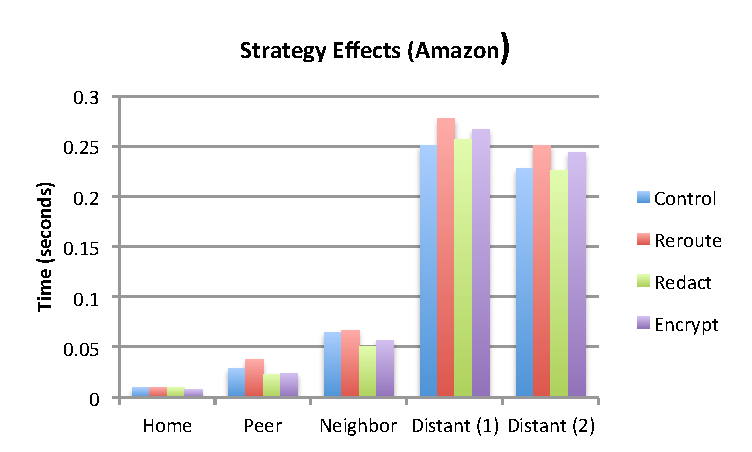
\includegraphics[width=6in]{strategy_effects_az}
\caption{Hierarchical Results from Amazon}
\label{fig:model:amazon-results}
\end{figure}

Figure ~\ref{fig:model:amazon-results} shows performance results from the Amazon testing node.  The access times for the content from the home, peer, and neighbor nodes were by far the smallest.  As the testing node was hosted in the same datacenter as these three nodes, that was to be expected.  The access times for both distant nodes was, however, surprisingly high.  With that in mind, the overall trend for response times is sensible however, with access time increasing as the requesting node is farther away from the content in the information network.  Queries from distant nodes need to traverse five information routers, while home, peer, and neighbor nodes only traverse one, two and three, respectively.  Also surprising was the finding that rerouting was generally more expensive from an availability perspective than encryption-based approaches.  This is likely attributable to the costs associated with attaching to the external SMTP server, hosted at Google, used as the out-of-band communications channel.  Also evident is remarkable performance variability.  Control data was collected at different times than experimental data, and infrastructural demands seem to have driven the control data availability to be less than that of other, managed approaches.  Overall, this evidence of variable performance due to external provider demands leads to the conclusion that overall, the availability costs of the various approaches are in fact negligible.

\begin{figure}[!t]
\centering
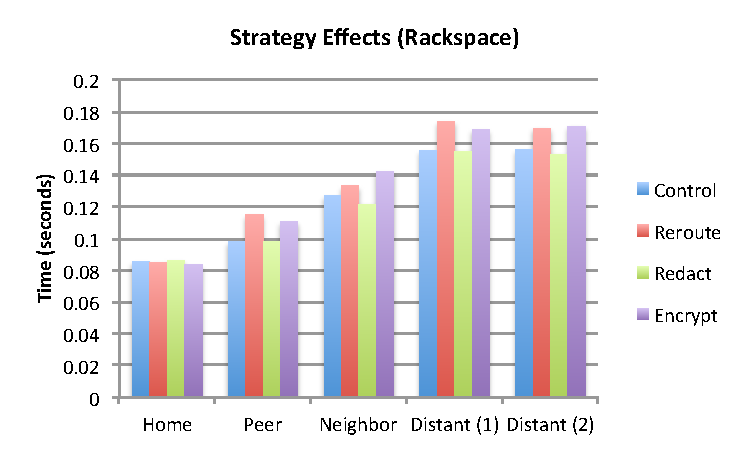
\includegraphics[width=6in]{strategy_effects_rs}
\caption{Hierarchical Results from Rackspace}
\label{fig:model:rackspace-results}
\end{figure}

Figure ~\ref{fig:model:rackspace-results} shows similar results to Figure ~\ref{fig:model:amazon-results}.  Here, the query times are much higher for the home and peer nodes, but actually lower for the distant nodes.  In this case, the content is still hosted in Amazon's infrastructure, but the testing node is at Rackspace.  As a result, the longer response time for content from the home node is to be expected.  Queries to distant nodes are actually shorter than the previous calls into distant nodes from Amazon.  This stems from the fact that the distant nodes are both hosted at Rackspace.  This locality shortens the round trip distance for a request.  Previously, from Amazon, a content request would need to travel from Amazon's east coast data centers to the Rackspace data center in Dallas, then back to the east coast for content, then back to Dallas, then back to the east coast.  In this test, the request only travels from Dallas to the east cost, and back.  Nevertheless, the overall performance profile is sensible, reflecting the expected shorter latency between home, peer, and neighbor nodes when compared to distant nodes.  Similar to amazon, cases when the control latency is higher than experimental latency emerge, indicating some amount of infrastructure performance variability.  In Figure ~\ref{fig:model:rackspace-results} however, it is evident that overall encryption and rerouting impact performance more than redacting, as would be expected.  Rerouting again has high overall impact, likely as a result of contacting Google's remote SMTP services.

Figure ~\ref{fig:model:comcast-results} Shows performance results measured from Comcast.  Interestingly, they show significant variability when accessing nodes hosted at Amazon, and more predictable performance when accessing nodes in Rackspace's infrastructure.  The overall variability does not follow the expected pattern of shorter response times when accessing content from nodes close to that content, except in a few cases.  This illustrates the kind of performance variability one can expect from an external service provider.

Integrity impacts are the result of approach rather than platform.  Redacting content destroys information integrity, as information is removed and not delivered to requesters.  Encryption maintains integrity the best of the three alternatives as information, even though encrypted, is still delivered, and delivered in the context of the query response at that.  Rerouting is better than redaction, in that sensitive information is still delivered, but worse than encryption, as it is not delivered within the response context and is sent out-of-band. Simulations removed sensitive information from the information network and dispatched it to a user's email address via SMTP over TLS when the selected strategy was rerouting.  This impacts information availability, as email delivery times can be highly variable.  In these experiments, delivery could take anything from a few seconds to a few minutes.

\begin{figure}[!t]
\centering
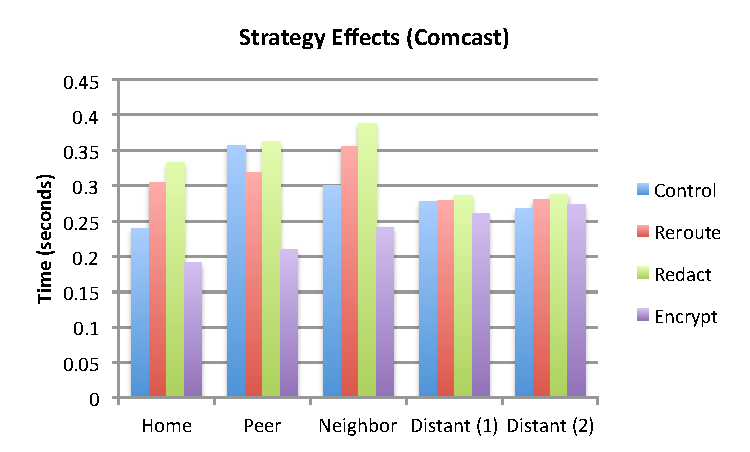
\includegraphics[width=6in]{strategy_effects_local}
\caption{Hierarchical Results from Comcast}
\label{fig:model:comcast-results}
\end{figure}

Confidentiality is likewise impacted primarily by approach and not by infrastructure.  Redacting sensitive content provides the best confidentiality protection, as sensitive content is simply not exposed.  Encryption is likely the worst solution from a confidentiality perspective as content encryption is a delaying tactic against a determined, well-resourced adversary.  Rerouting may be better or worse than encryption as an approach, depending on the confidentiality of the out-of-band channel.  If the security of that channel can be guaranteed, then it is likely a better approach.  If, on the other hand, the security of that channel is more variable or difficult to ascertain, encryption may be a more reliable approach.

Overall, results show that, from a performance perspective, the rerouting approach fares the worst, but only slightly, and certainly not in all cases.  Both results from Amazon and Rackspace, in Figures ~\ref{fig:model:amazon-results} and ~\ref{fig:model:rackspace-results}, show encryption as generally taking the second largest performance hit, just following rerouting.  Furthermore, network effects have a much larger impact on performance than information protection approaches.  The query to the home node is an excellent predictor of overall network stability, as content delivered directly from a home node is only subjected to the selected information protection strategy once.  Note that when queried from Amazon or Rackspace, the home node timing results are very close to uniform.  Queries from Comcast, however, are much more varied, indicating more highly variable quality of service within the Comcast network.  This is also supported by the gross distribution of response times.  Within both the Amazon and Rackspace networks, the farther a queried node is from the content requested, the worse the latency, as expected.  Comcast's network has a much more uniform information network response time overall as the processing time of the information network simulation is overshadowed by the highly varied performance of Comcast's physical network.  Availability is surprisingly uniform across all confidentiality strategies, showing little impact on end-to-end processing times.

\section{Non-Hierarchical Networks}
In order to test non-hierarchical networks, a simple branching network of participants was used, identical in form to the hierarchical network, though queries could be routed through the network from any point.  Queries could come into any node on the network, and would propagate through the network to the requested content, evaluating the returned content as it passes back through the network in response to the initial query.

In these experiments, the node that contains the content was queried, then the node immediately next to that content node, and so on, to a distance of five nodes.  The home node again contains content, and the additional nodes are marked by the distance in node count from the home node, starting with Neighbor (1), proceeding through Neighbor (5).  The non-hierarchical network was queried from Rackspace, Amazon, and Comcast, for a total of 250 queries per test, testing the system once per each confidentiality strategy.

\begin{figure}[!t]
\centering
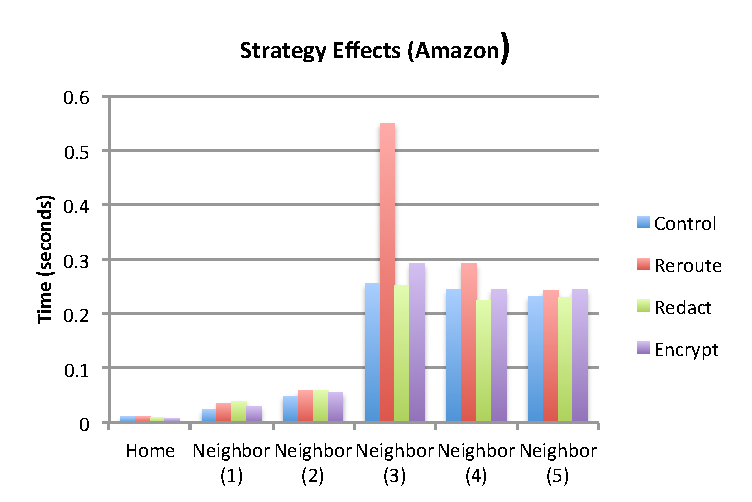
\includegraphics[width=6in]{nh_strategy_effects_az}
\caption{Non-Hierarchical Results from Amazon}
\label{fig:model:nh-amazon-results}
\end{figure}

Figure ~\ref{fig:model:nh-amazon-results} shows the performance of a non-hierarchical network as tested from the Amazon test node.  The content response latency is characteristic of moving farther from the source node through the network.  The request nodes switch from Amazon infrastructure to Rackspace infrastructure starting with Neighbor (3), and this is reflected in the sudden increase in latency.  As the tests originate from Amazon, at the Neighbor (3) node, a request and it's response must travel from Virginia to Texas, then back to Virginia, then back to Texas, then back to the original requester in Virginia.  The spike in latency at Neighbor (3) when re-routing traffic is caused by SMTP delays with systems hosted at Google.  Overall, the distribution is very similar to the hierarchical case.  Also evident is a continuation of the previous pattern in which re-routing is the least efficient strategy, followed by encryption, then redaction.

\begin{figure}[!t]
\centering
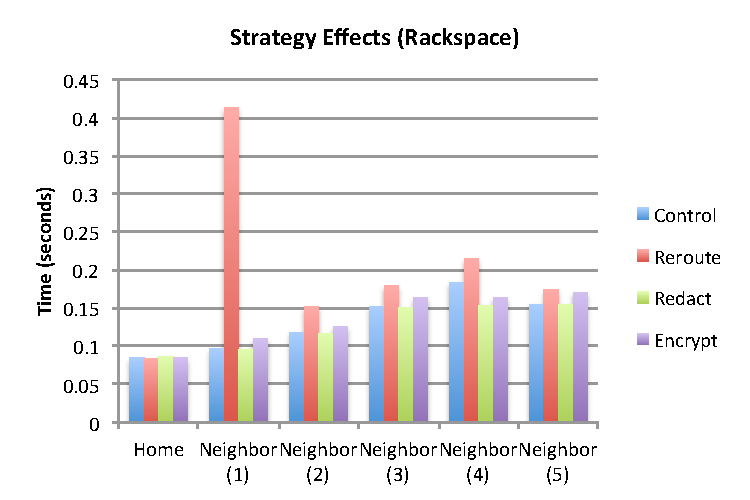
\includegraphics[width=6in]{nh_strategy_effects_rs}
\caption{Non-Hierarchical  Results from Rackspace}
\label{fig:model:nh-rackspace-results}
\end{figure}

Unlike the previous Amazon-based tests, the Rackspace tests shown in Figure ~\ref{fig:model:nh-rackspace-results} latencies seem much more uniform.  This again stems from the fact that each content query will always traverse the distance between Amazon and Rackspace data centers at least once.  Other than that, the distribution again shows an increase in measured latency as the queried node moves farther and farther away from the home node.  Once again, a dramatic spike in latency emerges based on SMTP delays when re-routing information.  The pattern of re-routing having the highest latency continues here as well.

\begin{figure}[!t]
\centering
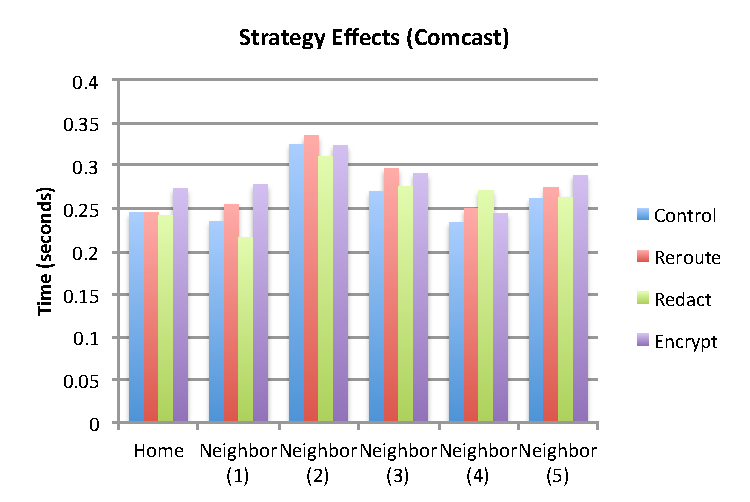
\includegraphics[width=6in]{nh_strategy_effects_local}
\caption{Non-Hierarchical Results from Comcast}
\label{fig:model:nh-comcast-results}
\end{figure}

Results from Comcast, included in Figure ~\ref{fig:model:nh-comcast-results}, shows a fairly regular distribution of response latencies overall.  In this case, the test node is ensconced within Comcast's network infrastructure.  Generally, re-routing is the least efficient approach, but not uniformly.  In this case, network effects created by the physical location of the testing node dominate these results.

Non-hierarchical networks behave very similarly to hierarchical networks.  This is not surprising --- although the nodes are more functionally complex, performing routing and repository functions, once the content is found and delivered the roles the nodes fall into mirror those in a hierarchical network.  For example, in a typical query, a node will receive a request, check the repository for the requested content, and if the content does not exist, pass the request onto the next known nodes.  This does differ slightly from the hierarchical case in that the nodes check for content at each routing step, though this is a very fast and simple test.  Once content is found, the response is routed back the the requester without any repository checks, just as it would be in a hierarchical system.

\section{Removing Network Effects}
Having established the parameters under which confidentiality strategies may be chosen, the next immediate area of concern involves the number of filtering events that can occur prior to a given information network suffering from degraded performance.  Previous results demonstrated that some kind of degradation of performance in the selected network based on distance from content does exist, but that can also be attributed to the distributed nature of the network itself.  Processing performance of a given node must be evaluated free of network effects in order to more clearly understand the availability implications of content filtering itself.

A single node, configured on one of the test nodes in either infrastructure, would yield the type of network effect free performance limits needed.  A node in Amazon's environments was configured such that requests were made of the home node itself, under each of the three confidentiality strategies.  Requests were also directed to the home node without any usage management systems engaged in order to collect control data.  After that initial request, the node was configured with various usage management strategies in order to measure their availability impact.

\begin{figure}[!t]
\centering
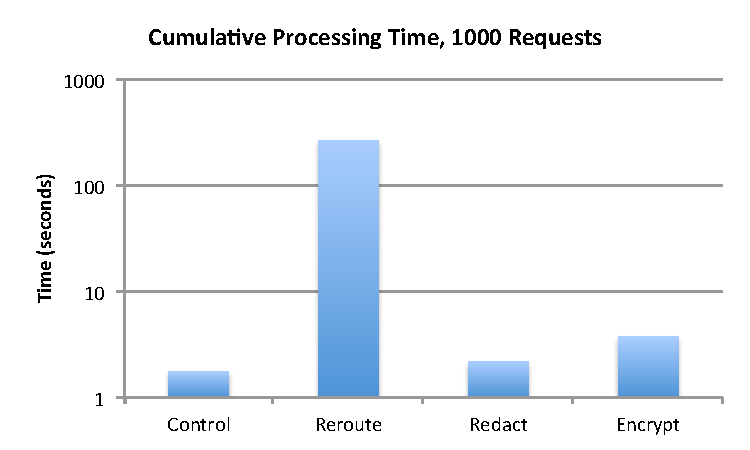
\includegraphics[width=6in]{single-node-results}
\caption{Results from Requests to a Singe Node}
\label{fig:model:single-node-results}
\end{figure}

As shown in Figure ~\ref{fig:model:single-node-results}, with information network effects removed, redaction and encryption have very similar performance overall.  Redaction, as a strategy, is very simple programmatically, and as symmetric encryption is used for information protection, ciphering and deciphering operations are very fast.  Rerouting, in this case, is clearly the worst strategy.  This is a result of the dependency of this strategy on external systems and system configuration times.  Specifically, configuring and using SMTP for each rerouting operation is prohibitively expensive.
%\input{content-slides/system}
%\section{System Architecture}
\begin{frame}
\frametitle{System Architecture}
What would this kind of overlay system look like?
\pause
\begin{itemize}
\item \textit{Meta-Model}
\pause
\item \textit{Non-Hierarchical Overlays}
\pause
\item \textit{Hierarchical Overlays}
\pause
\item \textit{Ontologies and Taxonomies}
\end{itemize}
\
\newline
\newline
\pause
\textit{...and what would the migration path to these systems look like?}
\end{frame}

\begin{frame}[t]
\frametitle{System Architecture - Level $\phi$}
\begin{figure}[!t]
\centering
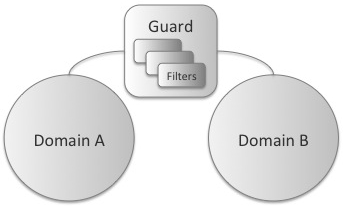
\includegraphics[width=2in]{model-phi-crop}
\label{fig:model:phi}
\end{figure}
This is a baseline cross-domain solution.  It is filter based and does not have any external  policy sources.  These are primarily:
\pause
\newline
\begin{itemize}
\item \textit{Filter-centric} --- They use content filters of some sort against submitted information.
\pause
\item \textit{Blacklist-oriented} --- They use hard-wired blacklists to filter and redact.
\end{itemize}
\end{frame}

\begin{frame}[t]
\frametitle{System Architecture - Level $\alpha$}
\begin{figure}[!t]
\centering
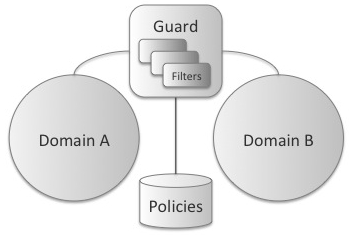
\includegraphics[width=2in]{model-alpha-crop}
\label{fig:model:alpha}
\end{figure}
This is a more advanced cross-domain solution featuring distributed policy management.  Characteristics include:
\pause
\newline
\begin{itemize}
\item {Generalized Control} --- No longer required to use fixed blacklist-centric solutions, these kinds of systems process policies defined over a more general ontology \footnote{Ontological impedance now a problem}.
\end{itemize}
\end{frame}

\begin{frame}[t]
\frametitle{System Architecture - Level $\beta$}
\begin{figure}[!t]
\centering
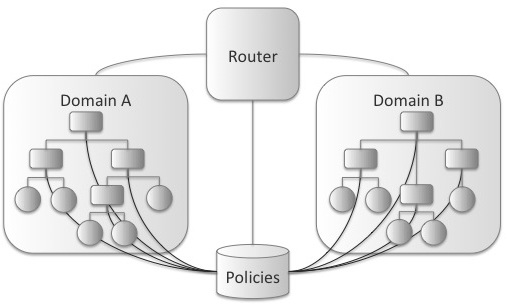
\includegraphics[width=2in]{model-beta-crop}
\label{fig:model:beta}
\end{figure}
We are beginning to inject usage management into the fabric of the network, linking content routing elements to policy information \footnote{Not really applicable to pure non-hierarchical systems}.
\newline
\pause
\begin{itemize}
\item \textit{Content-based Routing} --- We can start to implement content based routing at this point with available policy information.
\pause
\item \textit{Dynamic Context} --- We can also start to take advantage of changing network context with respect to routing data.
\end{itemize}
\end{frame}

\begin{frame}[t]
\frametitle{System Architecture - Level $\gamma$}
\begin{figure}[!t]
\centering
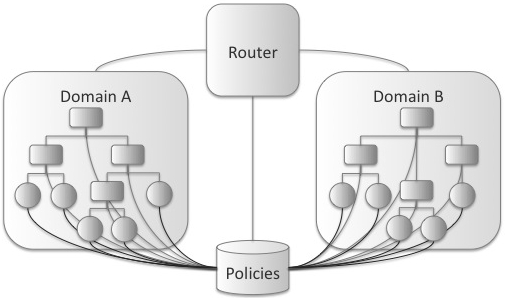
\includegraphics[width=2in]{model-gamma-crop}
\label{fig:model:gamma}
\end{figure}
We now are injecting usage management into every content node within the system.  This gives us:
\newline
\pause
\begin{itemize}
\item \textit{Extensive Control} --- We can now effectively do things like \textit{rights retraction}.
\pause
\item \textit{Pervasive Usage Management } --- We have content monitoring at all nodes of the content network.
\end{itemize}
\end{frame}

\begin{frame}[t]
\frametitle{System Architecture - Level $\delta$}
Here, we introduce the concept of a \textit{Smart License}:
\begin{itemize}
\pause
\item \textit{Mobile} --- Licenses are small programs that move along the overlay and are run at various policy enforcement points \cite{proposal:rfc3198}
\pause
\item \textit{Integrated} --- Content, Policies, Usage Management Mechanism all packaged in Smart License
\pause
\item \textit{Contained} --- Content and Policies are never exposed, all access to content is through specific interfaces
\end{itemize}
\pause
\begin{columns}[t]
\column{.5\textwidth}
\textit{Advantages}
\pause
\newline
\newline
Potentially more \textbf{secure} for content, provides finest-grained \textbf{control}; \textbf{simpler} routers and nodes
\column{.5\textwidth}
\textit{Disadvantages}
\pause
\newline
\newline
Mobile code requires \textbf{uniform execution environments}, which have their own \textbf{security} problems; \textbf{complex} license
\end{columns}
\end{frame}

\begin{frame}
\frametitle{Costs and Benefits}
So we have integrated usage management into a content network taking a very information-centric perspective.  At what cost?
\newline
\pause
\begin{columns}[t]
\column{.5\textwidth}
\textit{Costs}
\pause
\newline
\newline
Increasing \textbf{attack surface}; all these policy evaluation and injection points are nifty avenues for exploitation
\pause
\newline
\newline
Increasing \textbf{complexity}; dynamic routing makes things more difficult and expensive to manage
\column{.5\textwidth}
\textit{Benefits}
\pause
\newline
\newline
Additional \textbf{control} over sensitive content; both how it is \textbf{used} and how it is \textbf{distributed}
\pause
\newline
\newline
The ability to dynamically apply \textbf{new security controls} to transmitted information based on context (e.g. increase the strength of encryption)
\end{columns}
\end{frame}
%\section{Introduction}

\begin{frame}
\frametitle{Our Group and Current Work}
Our group has roots in digital rights management, machine learning and neural networks, and semantic analysis.
\pause
\newline
\newline
We are working on how to manage sensitive content in computer networks.  We are looking at three areas at this point:
\pause
\begin{itemize}
\item \textit{Routing} --- How can we control how sensitive information is routed over the internet? When and why is this appropriate, how can we do it, and where?
\pause
\item \textit{Redaction} --- If we dynamically redact information from transmitted content, what are the implications? how can we go about doing this?
\pause
\item \textit{Usage Management} --- After content has been redacted, how can we control content after delivery? when do we want to do this? why is it appropriate, and how can we implement this?
\end{itemize}
\pause
\begin{center}
\textbf{Simulations $\Rightarrow$ Cloud $\Rightarrow$ SDN (Openflow)}
\end{center}
\end{frame}

\begin{frame}
\frametitle{What We're Doing}
This is a sample of our preliminary work.  The accepted paper is six months old, and we've progressed since then.
\pause
\newline
\newline
Today I'm going to cover the submitted paper and touch on current progress as well.  This will involve:
\pause
\begin{itemize}
\item \textit{Covering Motivation and Current Work}
\pause
\item \textit{Describing Shortcomings of Current State}
\pause
\item \textit{Discussing Characteristics of Future Solutions}
\pause
\item \textit{Reviewing our Solution Taxonomy}
\pause
\item \textit{Discussing Simulations and Current Directions}
\end{itemize}
\begin{center}
\pause
\textbf{Please, any comments with respect to alternative avenues, collaboration, or resource pooling is more than welcome! That's why I'm here.}
\end{center}
\end{frame}

\begin{frame}
\frametitle{Introduction}
Distributed enterprise computing systems are facing a troubling future.  They are:
\pause
\begin{itemize}
\item \textit{Expensive} --- They do not use current commercial resources and use costly partitioning schemes
\pause
\item \textit{Unreliable} --- Too reliant on outmoded security approaches
\pause
\item \textit{Slow} --- Sensitive information is manually reviewed too often leading to the right people being unable to get the right information in time 
\end{itemize}
\
\newline
\pause
They need to be re-imagined to take advantage of radical shifts in computational provisioning.
\newline
\newline
\pause
\textit{Federal computer systems are a prime example of these kind of problematic distributed systems, and demonstrate the difficulty in implementing new technical solutions.}
\end{frame}
%\section{Motivation --- Cloud-centric Usage Management}

% Outline
% I. Frame the problem (use the AF proposal for this)
% II. Outline current solutions from UCDMO using guards
% III. Discuss problems (use pro/con list)
% IV. Frame specific challenges using slides II, III

\begin{frame}[t]
\frametitle{The Problems --- Customer Perspectives}
Current policy-centric systems are being forced to move to cloud environments and build much more open systems.  Usage management is a key problem in this domain --- information needs to be delivered to those who need it as soon as possible:
\newline
\newline
"...It is imperative to  effectively exchange information among components, Federal agencies, coalition partners, foreign governments and international organizations as a critical element of our efforts to defend the nation and execute national strategy..."\cite{proposal:info-sharing-strategy}
\newline
\begin{footnotesize}\textit{--- DoD Information Sharing Strategy}\end{footnotesize}
\newline
\newline
"...The CIO of the National Security Agency is focusing on IT architecture and a cloud-centric approach to sharing information..."\cite{proposal:nsa-cloud}
\newline
\begin{footnotesize}\textit{--- Informationweek}\end{footnotesize}
\end{frame}

\begin{frame}[t]
\frametitle{The Problem --- Characteristics}
Cloud systems may save money, provide more flexibility, but they also \cite{proposal:privacy-security-trust-cloud}:
\begin{itemize}
\item<2-> \textit{Are Not Private} --- User data control in SaaS is lacking, causing policy concerns for agencies; Data owners have no technical control over secondary use; providers may use offshore development; data can be routed across sensitive countries or secondarily stored on CDNs; data privacy on bankruptcy is ill-defined
\item<3-> \textit{Are Less Secure} --- Controlling data access, data may not be wiped in all XaaS scenarios, availability/backup leads to possible data proliferation, lack of standardization in intercloud communication and data transfer, multi-tenancy and side-channel attacks, difficult logging/auditing
\item<4-> \textit{Cannot Be Trusted} --- Trust relationships, consumer trust
\end{itemize}
\end{frame}

\begin{frame}[t]
\frametitle{Current Solutions}
How are these problems being addressed by impacted organizations?
\newline
\newline
\pause
They're just starting to be actively addressed and are an open research question \cite{proposal:assured-info-sharing}.
\newline
\newline
Cross-domain architectures are currently the standard for monitoring and information dissemination in an effort lead by the \textit{Unified Cross Domain Management Office}, associated with the Department of Defense (DoD) and the National Security Agency (NSA).
\end{frame}

\begin{frame}[t]
\frametitle{Current Solutions --- NSA}
Legacy cross-domain notional architecture \cite{proposal:nsa-arch}
\begin{figure}[!t]
\centering
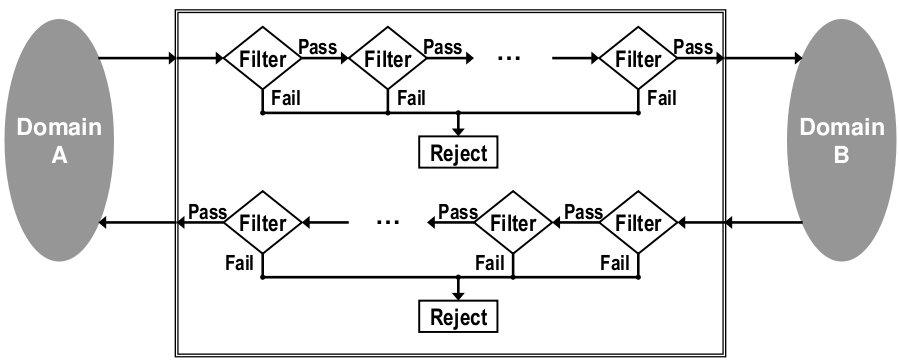
\includegraphics[width=3.4in]{nsa-legacy-arch}
\caption{NSA Legacy Model}
\label{fig:model:conceptual-model-nsa-legacy}
\end{figure}

\textit{Domain A} --- Private cloud managed by the Air Force
\newline
\textit{Domain B} --- A public operational network
\end{frame}

\begin{frame}[t]
\frametitle{Current Solutions --- NSA (SoA)}
Future cross-domain notional architecture \cite{proposal:nsa-arch}
\begin{figure}[!t]
\centering
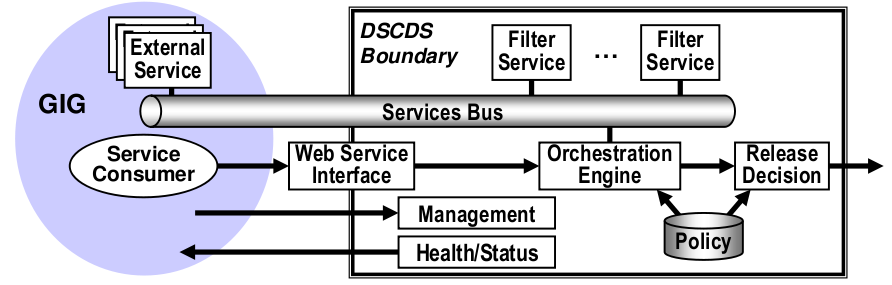
\includegraphics[width=3.4in]{nsa-arch}
\caption{NSA Service-Oriented Model}
\label{fig:model:conceptual-model-nsa}
\end{figure}

\textit{GiG} --- Global Information Grid; a large public cloud operated by the DoD
\newline
\textit{DSCDS} --- Distributed Service-oriented Cross Domain Solution
\end{frame}

\begin{frame}[t]
\frametitle{Current Solutions --- Raytheon}
Raytheon's notional architecture supporting cross-domain information flow \cite{proposal:raytheon-arch}:
\begin{figure}[!t]
\centering
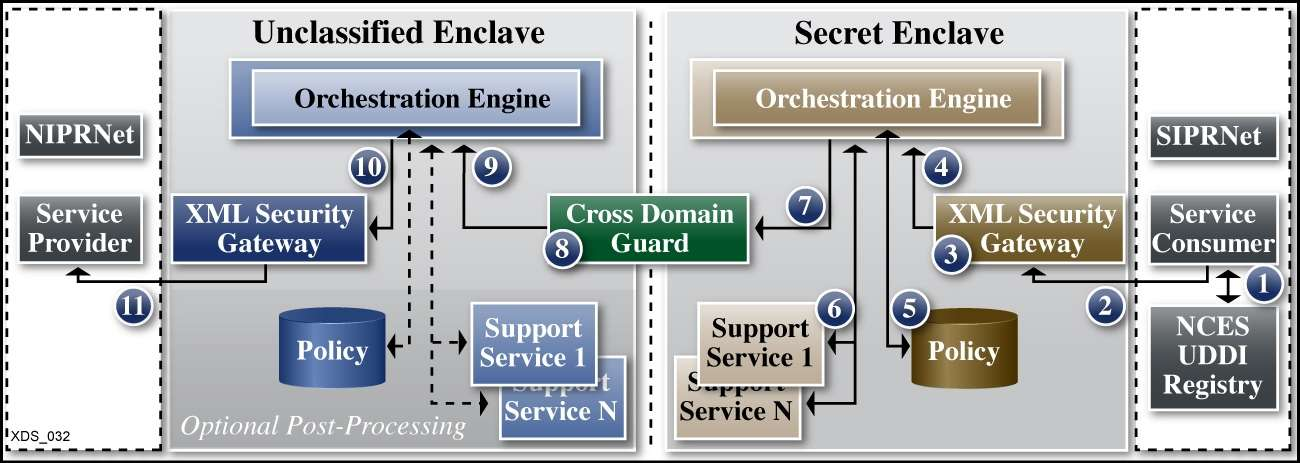
\includegraphics[width=3.4in]{raytheon-arch}
\caption{Raytheon Model}
\label{fig:model:conceptual-model-raytheon}
\end{figure}

\textit{...still uses a single perimeter guard...}
\end{frame}

\begin{frame}[t]
\frametitle{Current Solutions --- BAH}
{Booz$\mid$Allen$\mid$Hamilton} presented a service-centric cross domain solution in 2009 \cite{proposal:bah-arch}:
\begin{figure}[!t]
\centering
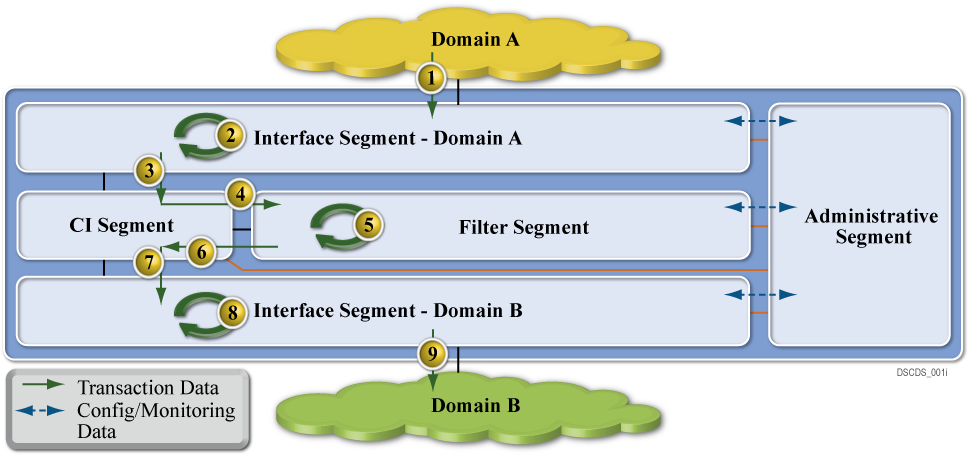
\includegraphics[width=3.4in]{bah-arch}
\caption{Booz|Allen|Hamilton Model}
\label{fig:model:conceptual-model-bah}
\end{figure}
\textit{...still uses a single perimeter guard (called a filter segment)...}
\end{frame}

\begin{frame}[t]
\frametitle{Future Solution}
Organizations are falling back on what they know in the scope of new problems.
\begin{figure}[!t]
\centering
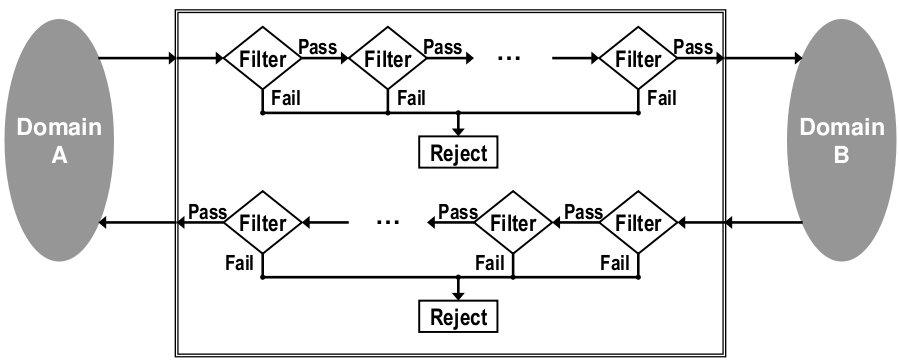
\includegraphics[width=3.4in]{nsa-legacy-arch}
\caption{NSA Legacy Model}
\label{fig:model:conceptual-model-nsa-legacy-II}
\end{figure}
Even though we know they don't work \cite{proposal:ron-ross}.
\end{frame}

%overlay:
%- Policy into network fabric
%- Multiple compartments on same physical network
%- Network can integrate cloud components securely
%- Provides security in depth
%
%traditional/guard:
%- Policy centralized single points of failure
%- Each physical network can only be at one compartment level
%- Use is tied to the physical network; no cloud integration possible
%- Boundary security only 
\begin{frame}
\frametitle{Characteristics of Current Solutions}
\begin{itemize}
\item<2-> \textit{Centralized Policy} --- They use centralized policy injection into communication flow.  Note that in each sample model, policy is \textit{only} evaluated at guard points.
\item<3-> \textit{Physical to Compartment Mapping} --- In each of these cases, users are only allowed to exchange one type of information per domain.  The physical domain systems are locked (by operational policy) to a single classification level limit.  Users cannot, for example, have \emph{Top Secret} material on a network accredited for \emph{Secret} material.
\item<4-> \textit{Perimeter Protection} --- The use of a single policy enforcement point at domain interconnects supplies a crunchy exterior to the creamy interior data filling.
\end{itemize}
\end{frame}

\begin{frame}
\frametitle{What's Wrong with Current Solutions?}
\begin{itemize}
\item<2-> \textit{Centralized Policy} --- A centralized policy enforcement system simplifies infrastructural attacks.  Adversaries know exactly where to focus efforts to compromise policy enforcement, lowering overall system trustworthiness and reliability. 
\item<3-> \textit{Physical to Compartment Mapping} --- The traditional model for multi-level security, enforced in this scheme, is that the network is classified at the level of the most sensitive data that transits it.  Ergo, those that have clearances at a level to view sensitive data are unable to view that data generally without extensive swivel-chair integration.
\item<4-> \textit{Perimeter Protection} --- Perimeter protection is a necessary but not sufficient security approach.  By itself, it doesn't work \cite{proposal:ron-ross}.
\end{itemize}
\end{frame}

\begin{frame}
\frametitle{Characteristics of Future Solutions}
\begin{itemize}
\item<2-> \textit{Decentralized Policy} --- Policy management is decentralized and integrated within the fabric of the system.  The system is both more secure and resilient as a result, better able to control information and operate under stressful conditions.
\item<3-> \textit{Infrastructure Reuse} --- Multi-tenancy can lower costs and increase reliability and is furthermore a common attribute of cloud systems.  An appropriately secured system facilitates integration of computing resources into multi-tenant environments.
\end{itemize}
\end{frame}

\begin{frame}
\frametitle{Characteristics of Future Solutions}
\begin{itemize}
\item<2-> \textit{Cloud Integration} --- The ability to handle multi-tenant environments and to reliably secure both data at rest and data in motion leads to computational environments deployable in cloud systems.
\item<3-> \textit{Security in Depth} --- Systems must operate under \textit{all} conditions, including when they are under attack or compromise \cite{proposal:ron-ross}.  Ergo, they must provide protection to sensitive data in depth.
\end{itemize}
\end{frame}


%\section{Progress}

\begin{frame}
\frametitle{Initial Prototype}
\begin{figure}
\centering
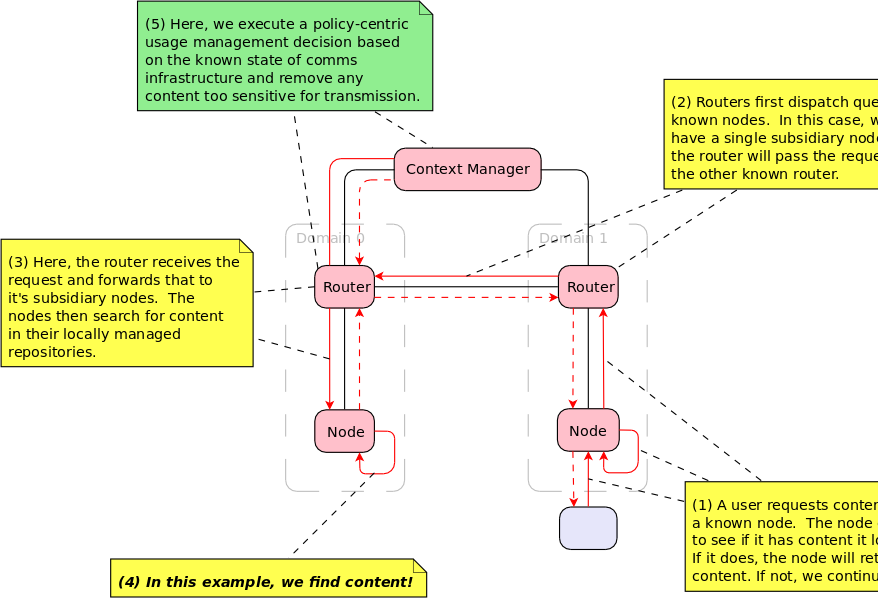
\includegraphics[width=4in]{cross-domain-prototype}
\label{fig:implementation:prototype}
\end{figure}
\end{frame}

\begin{frame}
\frametitle{Current Work}
We're currently extending the local simulation to a distributed content system.  The environment we're using consists of roughly 40 nodes distributed over Rackspace (using Rackspace Servers), Amazon (using EC2), and our local Eucalyptus installation.  We will use Heroku as well (We're deliberately building networks over providers and mixing IAAS and PAAS).
\newline
\pause
\begin{itemize}
\item \textit{Ruby} --- We use Ruby and the Ruby runtime as our base runtime engine.  We use associated tools like RVM, Gem, and Bundler to manage our projects.
\pause
\item \textit{Sinatra} --- Sintara is a simple but powerful HTTP engine.
\pause
\item \textit{Capistrano} --- Capistrano simplifies deployment of software on large numbers of nodes.
\pause
\item \textit{YAML} --- YAML is a simple data serialization language.
\end{itemize}
\end{frame}

\begin{frame}[c]
\frametitle{Future Work}
We are in the process of configuring infrastructure to begin work with Openflow-enabled hardware.  We will use Ruby and Ruby tools in this environment as well, with the addition of Trema, a Ruby and C based environment for building Openflow controllers.
\end{frame}

\begin{frame}[c]
\begin{center}
\textbf{Questions? Comments?}
\end{center}
\end{frame}

%\section{References}
\begin{frame}
\def\newblock{}
\tiny{
\bibliographystyle{abbrv}
\bibliography{bib/proposal}}
\end{frame}

\end{document}

